%
% This template has been created by Theo J. Mertzimekis, PhD
% It can be modified freely to meet your needs.
% Help in using this thesis can be found here:
% http://users.uoa.gr/~tmertzi/LaTeX
%
% As a minimal credit to the creator, please do not remove the lines above
%
\documentclass[12pt]{report}

% package to activate greek language - the sequence languages appear below is IMPORTANT!!!
\usepackage[greek,english]{babel}
\usepackage{varioref}
%\usepackage{hyperref}
\usepackage{multicol}
% package to handle graphics
\usepackage{graphicx}
% package to handle multiple figures in a minipage
\usepackage{subfigure}
% package to extend math capabilities
\usepackage{amsmath,amssymb,isotope}
\newcommand{\Lagr}{\mathcal{L}}
\usepackage[version=4]{mhchem}

%package to activate XeTeX font manager
\usepackage{fontspec}
\usepackage{physics}

% DOCUMENT LAYOUT
\usepackage{geometry} 
\geometry{a4paper, textwidth=5.5in, textheight=8.5in, marginparsep=7pt, marginparwidth=.6in}
%\geometry{a4paper}
\setlength\parindent{8mm}
\setlength\parskip{5mm}

% FONTS
\usepackage{xunicode}
\usepackage{xltxtra}
\usepackage{xcolor}
\defaultfontfeatures{Mapping=tex-text} % converts LaTeX specials (``quotes'' --- dashes etc.) to unicode
%\setromanfont [Ligatures={Common}, BoldFont={GFS Artemisia Bold}, ItalicFont={Gentium Italic}]{Gentium}
%\setmonofont[Scale=0.8]{Monaco} 
\setmainfont{Times New Roman} % You can set your main font here.

% ---- CUSTOM AMPERSAND
\newcommand{\amper}{{\fontspec[Scale=.95]{Gentium Italic}\selectfont\itshape\&}}

% package to handle line spacing
\usepackage{setspace}

% HEADINGS
\usepackage{sectsty} 
\usepackage[normalem]{ulem} 
\sectionfont{\rmfamily\mdseries\upshape\Large}
\subsectionfont{\rmfamily\bfseries\upshape\normalsize} 
\subsubsectionfont{\rmfamily\mdseries\upshape\normalsize} 

% PDF SETUP
% ---- FILL IN HERE THE DOC TITLE AND AUTHOR

%add dots to content
\usepackage{subfigure}
\usepackage[subfigure]{tocloft}
\renewcommand{\cftchapleader}{\cftdotfill{\cftdotsep}}

%setup colors in cite, links, etc..
\usepackage[driverfallback=dvipdfmx, bookmarks, colorlinks, breaklinks, pdftitle={Georgios K. Simopoulos},pdfauthor={gsimop}]{hyperref}  
\hypersetup{linkcolor=black,citecolor=blue,filecolor=black,urlcolor=blue} 

% package for fancy style headers and footers
\usepackage{fancybox}


% redefine bullet symbols and section style
\renewcommand\thesection{\arabic{section}.}
\renewcommand{\labelitemi}{$\blacktriangleright$}
\renewcommand{\labelitemii}{$\bullet$}

% change captions especially for greek language - if the document is in ENGLISH, they should vanish
\addto\captionsenglish{%
  \renewcommand\prefacename{Πρόλογος}%
  \renewcommand\refname{Αναφορές}%
  \renewcommand\abstractname{Περίληψη}%
  \renewcommand\bibname{Βιβλιογραφία}%
  \renewcommand\chaptername{Chapter}%
  \renewcommand\appendixname{Παράρτημα}%
  \renewcommand\contentsname{Contents}%
  \renewcommand\listfigurename{Κατάλογος Σχημάτων}%
  \renewcommand\listtablename{Κατάλογος Πινάκων}%
  \renewcommand\indexname{Ευρετήριο}%
  \renewcommand\figurename{Σχήμα}%
  \renewcommand\tablename{Πίνακας}%
  \renewcommand\partname{Μέρος}%
  \renewcommand\enclname{Συνημμένα}%
  \renewcommand\ccname{Κοινοποίηση}%
  \renewcommand\headtoname{Προς}%
  \renewcommand\pagename{Σελίδα}%
  \renewcommand\seename{βλέπε}%
  \renewcommand\alsoname{βλέπε επίσης}%
  \renewcommand\proofname{Απόδειξη}%
  \renewcommand\glossaryname{Γλωσσάρι}%
  }

\usepackage{xgreek}

%myedit
\newcommand{\Fourier}{\mathcal{F}}
\usepackage[labelfont=bf,font={footnotesize,it}]{caption}
\usepackage{scalerel}
%Includes "References" in the table of contents
\usepackage[nottoc]{tocbibind}

\renewcommand\thesection{\arabic{section}}
%    \renewcommand\theequation{\thesection.\arabic{equation}}
%     \renewcommand\thesubsubsection{\thesubsection.\arabic{subsubsection}}
\usepackage{mathtools}

\usepackage{tensor}

\DeclareMathOperator{\sinc}{sinc}

%%%%%%%%% END OF PREAMBLE %%%%%%%%%%%%

\begin{document}

\setlanguage{greek} %% this is to activate greek hyphenation

% make title out of \author, \title, \date  specified in the preamble

% create a blank page immediately after the cover page

\begin{titlepage}
%
%

\vspace{10mm}


\begin{center}
{\large \textsc{Special topics in photonics}}\\[3\baselineskip]


 % Tagline or further description
{\noindent\Huge\bfseries
Solutions of the problem sheets
}\\[\baselineskip] % Title



{\Large Georgios Simopoulos}\\[\baselineskip] % Author name
{\small Professors: K.Makris, D.Psaltis }\\[3\baselineskip] % Author name


{\noindent Heraklion 2023}\\[\baselineskip]
\end{center} % Publisher and logo

%
%
\end{titlepage}
\pagebreak
% Create table of contents - not mandatory
\tableofcontents
\include{blank_page}

% Create a list of figures - not mandatory
%\listoffigures

% include files with content. Changes the names according to your taste.


\setlength{\fboxsep}{0pt}
\setlength{\fboxrule}{.1pt}
%%\[ \fbox{$\Box$} \fbox{$\hat\Box$} \fbox{$\tilde\Box$} \]



\chapter{FFT}
\section{Problem set 1}
\subsection{Problem 1}

\begin{flushleft}
Με $f(x)=e^{-a|x|}$:
\begin{align*}
\mathcal{F}[f(x)]&= \int_{-\infty}^{\infty} f(x) e^{ik x}dx=\int_{-\infty}^{\infty}e^{-a|x|}e^{ik x}dx=\int_{-\infty}^{0} e^{ax}e^{ik x}dx + \int_{0}^{\infty}e^{-ax}e^{ik x} dx\\&= \frac{1}{a+ik}e^{(a+ik)x}\Biggr|_{-\infty}^{0}-\frac{1}{a-ik}e^{-(a-ik)x}\Biggr|_{0}^{\infty}=\frac{1}{a+ik}+\frac{1}{a-ik}=\frac{2a}{a^{2}+k^{2}}
\end{align*}
\end{flushleft}

\begin{figure}[htp]
\centering
\vstretch{1}{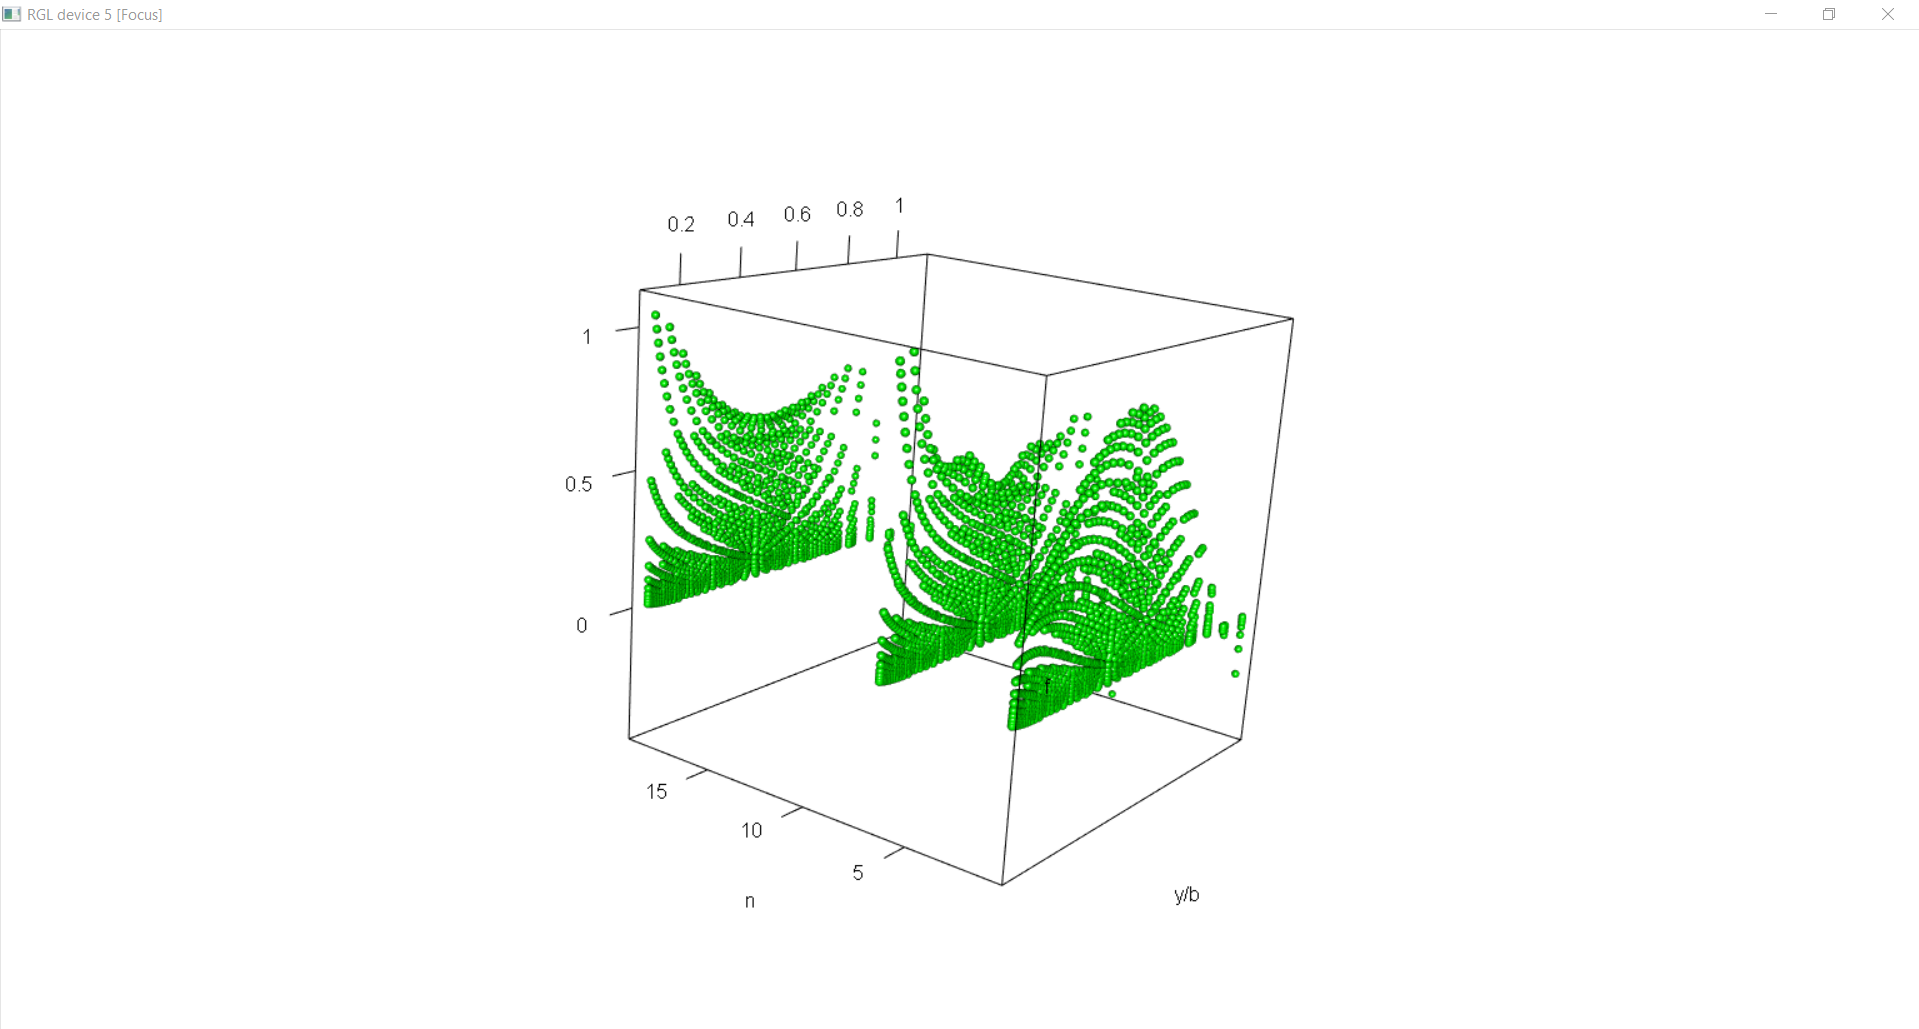
\includegraphics[scale=0.4]{Screenshot_1.jpg}}\caption{FFT στην συνάρτηση $f(x)=e^{-a|x|}$}\label{fig:1}
\end{figure}


\newpage

\begin{figure}[htp]
\centering
\vstretch{1}{\includegraphics[scale=0.4]{Screenshot_2.jpg}}\caption{Στο αριστερό διάγραμμα γίνεται σύγκριση αναλυτικής με αριθμητικής Fourier transformed συνάρτηση στην συνάρτηση $f(x)=e^{-a|x|}$, ενώ στο δεξί παρατίθεται η ποσοτική διαφορά των δύο αυτών.}\label{fig:2}
\end{figure}
\clearpage


\subsection{Problem 2}

\begin{itemize}
\item 1D

Με $f(x)=e^{-ax^{2}}$ και με τη χρήση του ολοκληρώματος Gauss:
\begin{align*}
\mathcal{F}[f(x)]&= \int_{-\infty}^{\infty} f(x) e^{ik x}dx=\int_{-\infty}^{\infty}e^{-ax^{2}}e^{ik x}dx\\&= \int_{-\infty}^{\infty} e^{-a(x^{2}-i\frac{k}{a}x-\frac{k^{2}}{4a^{2}})}e^{-\frac{k^{2}}{4a}}  dx\\&=e^{-\frac{k^{2}}{4a}}\int_{-\infty}^{\infty} e^{-a(x-i\frac{k}{2a})^{2}}dx \\&=e^{-\frac{k^{2}}{4a}}\int_{-\infty}^{\infty} e^{-ax'}dx '=e^{-\frac{k^{2}}{4a}}\sqrt{\frac{\pi}{a}}
\end{align*}

\newpage

\begin{figure}[htp]
\centering
\vstretch{1}{\includegraphics[scale=0.35]{Screenshot_3.jpg}}\caption{FFT στην συνάρτηση $f(x)=e^{-ax^{2}}$}\label{fig:3}
\end{figure}

\begin{figure}[htp]
\centering
\vstretch{1}{\includegraphics[scale=0.35]{Screenshot_4.jpg}}\caption{Στο αριστερό διάγραμμα γίνεται σύγκριση αναλυτικής με αριθμητικής Fourier transformed συνάρτηση στην συνάρτηση $f(x)=e^{-ax^{2}}$, ενώ στο δεξί παρατίθεται η ποσοτική διαφορά των δύο αυτών.}\label{fig:4}
\end{figure}

\clearpage

\item 2D

Με $f(x,y)=e^{-a(x^{2}+y^{2})}=f(x)f(y)$ και πάλι με τη χρήση του ολοκληρώματος Gauss:
\begin{align*}
\mathcal{F}[f(x,y)]&=\int_{-\infty}^{\infty}\int_{-\infty}^{\infty}f(x,y)e^{i(k_{x}x+k_{y}y)}dxdy\\&=\int_{-\infty}^{\infty}f(x)e^{ik_{x}x}dx \int_{-\infty}^{\infty}f(y)e^{ik_{y}y}dy\\&= e^{-\frac{k_{x}^{2}}{4a}}e^{-\frac{k_{y}^{2}}{4a}}\sqrt{\frac{\pi}{a}}\sqrt{\frac{\pi}{a}}=\frac{\pi}{a}e^{-\frac{1}{4a}(k_{x}^{2}+k_{y}^{2})}
\end{align*}



\begin{figure}[htp]
\centering
\vstretch{1}{\includegraphics[scale=0.45]{Screenshot_6.jpg}}\caption{Στο αριστερό διάγραμμα φαίνεται η αριθμητική Fourier transformed συνάρτηση μέσω FFT στην συνάρτηση $f(x)=e^{-a(x^{2}+y^{2})}$, ενώ στο δεξί διάγραμμα φαίνεται η αναλυτική Fourier transformed συνάρτηση στην συνάρτηση $f(x)=e^{-a(x^{2}+y^{2})}$}\label{fig:6}
\end{figure}

\newpage

\begin{figure}[htp]
\centering
\vstretch{1}{\includegraphics[scale=0.8]{Screenshot_7.jpg}}\caption{ Παρατίθεται η ποσοτική διαφορά της αναλυτικής με την αριθμητική λύση ΜΧ Fourier.}\label{fig:7}
\end{figure}



\end{itemize}



\subsection{Problem 3}

Σημείωση: ο ορισμός της κανονικοποιημένης συνάρτησης $\sinc(x)\equiv \frac{sin(\pi x)}{\pi x}$, ενώ ο ορισμός της μή κανονικοποιημένης είναι $sinc(x)\equiv \frac{sin(x)}{x}$. Ενώ στις πράξεις παρακάτω εφαρμόζουμε τον μη κανονικοποιημένο ορισμό, στα Matlab προγραμματάκια χρειάζεται η κανονικοποιημένη συνάρτηση, επομένως η διαφορά των δύο φαίνεται απλώς με έναν μετασχηματισμό $k\rightarrow \frac{k}{\pi}$:
\begin{align*}
\sinc(ka)&=\frac{\sin(ka)}{k}= \frac{\sin(\frac{k}{\pi}a\pi)}{\frac{k}{\pi}\pi}=\frac{\sin(k'a\pi)}{k'\pi}\equiv \sinc_{norm}(k'a)
\end{align*}

\begin{itemize}
\item 1D

Με $f(x)=1$, $x\in [-a,a]$ και $f(x)=0$ αλλού, θα έχουμε:

\begin{align*}
\mathcal{F}[f(x)]&= \int_{-\infty}^{\infty} f(x) e^{ik x}dx = \int_{-a}^{a} e^{ik x}dx =\frac{1}{ik}2i \sin(k a)=\frac{2\sin(k a)}{k}=2a\sinc(ka)
\end{align*}

\newpage

\begin{figure}[htp]
\centering
\vstretch{1}{\includegraphics[scale=0.4]{Screenshot_8.jpg}}\caption{FFT στην συνάρτηση $f(x)=rectangularPulse$ σε 1Δ}\label{fig:8}
\end{figure}

\begin{figure}[htp]
\centering
\vstretch{1}{\includegraphics[scale=0.4]{Screenshot_9.jpg}}\caption{Στο αριστερό διάγραμμα γίνεται σύγκριση αναλυτικής με αριθμητικής Fourier transformed συνάρτηση στην συνάρτηση $f(x)=rectangularPulse$, ενώ στο δεξί παρατίθεται η ποσοτική διαφορά των δύο αυτών.}\label{fig:9}
\end{figure}

\clearpage

\item 2D

Με $f(x,y)=1$, $x\in [-a,a]$,$y\in [-a,a]$ και $f(x,y)=0$ αλλού, θα έχουμε:

\begin{align*}
\mathcal{F}[f(x,y)]&=\int_{-\infty}^{\infty}\int_{-\infty}^{\infty} f(x,y) e^{i(k_{x} x+k_{y} y)}dxdy\\&= \int_{-a}^{a} e^{ik_{x} x}dx \int_{-a}^{a} e^{ik_{y} y}dy\\&= \frac{4}{k_{x}k_{y}} \sin(k_{x}a)\sin(k_{y}a)=4a^{2}\sinc(k_{x}a)\sinc(k_{y}a)
\end{align*}


\begin{figure}[htp]
\centering
\vstretch{1}{\includegraphics[scale=0.7]{Screenshot_10.jpg}}\caption{Η συνάρτηση $f(x,y)=rectangularPulse$ σε 2Δ}\label{fig:10}
\end{figure}

\newpage

\begin{figure}[htp]
\centering
\vstretch{1}{\includegraphics[scale=0.35]{Screenshot_11.jpg}}\caption{Σύγκριση αναλυτικής (δεξιά) με αριθμητικής (αριστερά) Fourier transformed συνάρτηση στην συνάρτηση $f(x,y)=rectangularPulse$ σε 2Δ}\label{fig:11}
\end{figure}



\begin{figure}[htp]
\centering
\vstretch{1}{\includegraphics[scale=0.45]{Screenshot_12.jpg}}\caption{ Σύγκριση αναλυτικής με αριθμητικής Fourier ποσοτικά}\label{fig:12}
\end{figure}
\clearpage

\end{itemize}







\end{document}